\documentclass[a0,portrait]{a0poster}

\usepackage{multicol} % This is so we can have multiple columns of text side-by-side
\columnsep=100pt % This is the amount of white space between the columns in the poster







\columnseprule=0pt % This is the thickness of the black line between the columns in the poster

\usepackage[svgnames]{xcolor} % Specify colors by their 'svgnames', for a full list of all colors available see here: http://www.latextemplates.com/svgnames-colors

\usepackage{times} % Use the times font
%\usepackage{palatino} % Uncomment to use the Palatino font

\usepackage{dsfont}
\usepackage{tcolorbox}
\usepackage{graphicx} % Required for including images
\graphicspath{{figures/}} % Location of the graphics files
\usepackage{booktabs} % Top and bottom rules for table
\usepackage[font=small,labelfont=bf]{caption} % Required for specifying captions to tables and figures
\usepackage{amsfonts, amsmath, amsthm, amssymb} % For math fonts, symbols and environments
\usepackage{wrapfig} % Allows wrapping text around tables and figures
\usepackage{graphicx}
\usepackage[T1]{fontenc}
\usepackage{lmodern} 

    
\begin{document}

\newcommand{\bra}[1]{\langle #1|}

\newcommand{\ket}[1]{|#1\rangle}

\newcommand{\braket}[2]{\langle #1|#2\rangle}

%----------------------------------------------------------------------------------------
%	POSTER HEADER 
%----------------------------------------------------------------------------------------

% The header is divided into two boxes:
% The first is 75% wide and houses the title, subtitle, names, university/organization and contact information
% The second is 25% wide and houses a logo for your university/organization or a photo of you
% The widths of these boxes can be easily edited to accommodate your content as you see fit

\begin{minipage}[b]{0.75\linewidth}
\veryHuge \color{NavyBlue} \textbf{Track Reconstruction with ATLAS Upgrade Prototypes using the General Broken Lines Algorithm within EUTelescope} \color{Black}\\ \vspace{1cm} % Title
%\Huge\textit{Track Reconstruction with ATLAS Upgrade Prototypes using the General Broken Lines Algorithm within EUTelescope}\\[2cm] % Subtitle
\huge \textbf{Alexander Morton}\\[0.5cm] % Author(s)
\huge University of Glasgow, School of Physics \& Astronomy, \\ Partice Physics Experimental\\[0.4cm] % University/organization
\Large \texttt{a.morton.2@research.gla.ac.uk}
\end{minipage}
%
\begin{minipage}[b]{0.25\linewidth}

\includegraphics[width=20cm]{GlaUni.png}\\

\includegraphics[width=7cm]{mp2-logo.png} \hspace{3cm} 
\includegraphics[width=7cm]{gbl-logo.png}\\
\end{minipage}

\vspace{1cm} % A bit of extra whitespace between the header and poster content

%----------------------------------------------------------------------------------------

\begin{multicols}{2} % This is how many columns your poster will be broken into, a portrait poster is generally split into 2 columns

%----------------------------------------------------------------------------------------
%	ABSTRACT
%----------------------------------------------------------------------------------------

\begin{tcolorbox}
\color{Navy} % Navy color for the abstract

\begin{abstract}
The General Broken Lines (GBL) algorithm has been successfully integrated into the EUTelescope framework. This is designed to be a generic fitter for many different testbeam setups. Many datasets have been successfully reconstructed and all examples can be found installed with EUTelescope by default. A subset of these are ATLAS upgrade inner tracker prototypes. These prototypes are a variety of strip and pixel sensors which have been tested at the DESY/SLAC testbeam. 


\end{abstract}
\end{tcolorbox}

%----------------------------------------------------------------------------------------
%	INTRODUCTION
%----------------------------------------------------------------------------------------



\begin{tcolorbox}
\color{DarkSlateGray} % DarkSlateGray color for this section

\section*{Background}

\subsection*{Fitting with GBL and Alignment}
EUTelescope is a highly generic testbeam reconstruction and analysis framework\cite{eutel}. The GBL algorithm is mathematically equivalent to a Kalman filter but computationally different \cite{claus1}. It solves the above problem in terms of offsets of each GBL point and then relating this back to the usual track parameters. This allows the track solution to be found far more easily. Millepede is an algorithm used for alignment which relies to splitting the problem into global parameters(Alignment parameters, X shifts for example) and local parameters (Each track parameter, position on a plane for example)\cite{blobel}. Both GBL and Millipede are employed for track reconstruction. This process begins at pattern recognition and then using five step reconstructs the tracks and adds the information needed to align the detector planes. 
Pattern recognition is needed to identify the hits which make up a track. Two different forms of pattern recognition exist for use with GBL
\begin{itemize}
\item \textbf{Clustering} Propagate all hits to the first plane and cluster. 
\item \textbf{Triplets} Associate two hits together to form doublet track and three to form triplet. Continue association to create final track.
\end{itemize}

The GBL track fitting and alignment comes in five steps:
\begin{itemize}
\item Link GBL points together to form a complete track described by discrete points.
Figure \ref{Scat} shows the linking of GBL point together. It consists of linking measurement/scattering errors using the initial trajectory parametrised.
\item Points which correspond to hits have measurements added with errors. The red points on the green plane of figure \ref{Scat} show these points on the green planes. The measurements pull the track towards it if included in fit.
\item Points with model scattering have kink angles and errors added. The orange points on figure \ref{Scat} show these points. These points allow a kink to be formed relative to the track incidence at that point.
\item Global derivatives which relate motions of the sensors with local frame residuals are added for alignment.
Any relation between the residual on each plane and parameters for the full system. Used in alignment.
\item Local derivatives are added to determine parameters which relate to tracks residual. Useful for kink angle estimations.
\end{itemize}

This information is needed for all track fitting and alignment, apart from the local derivatives.

\end{tcolorbox}
\begin{center}
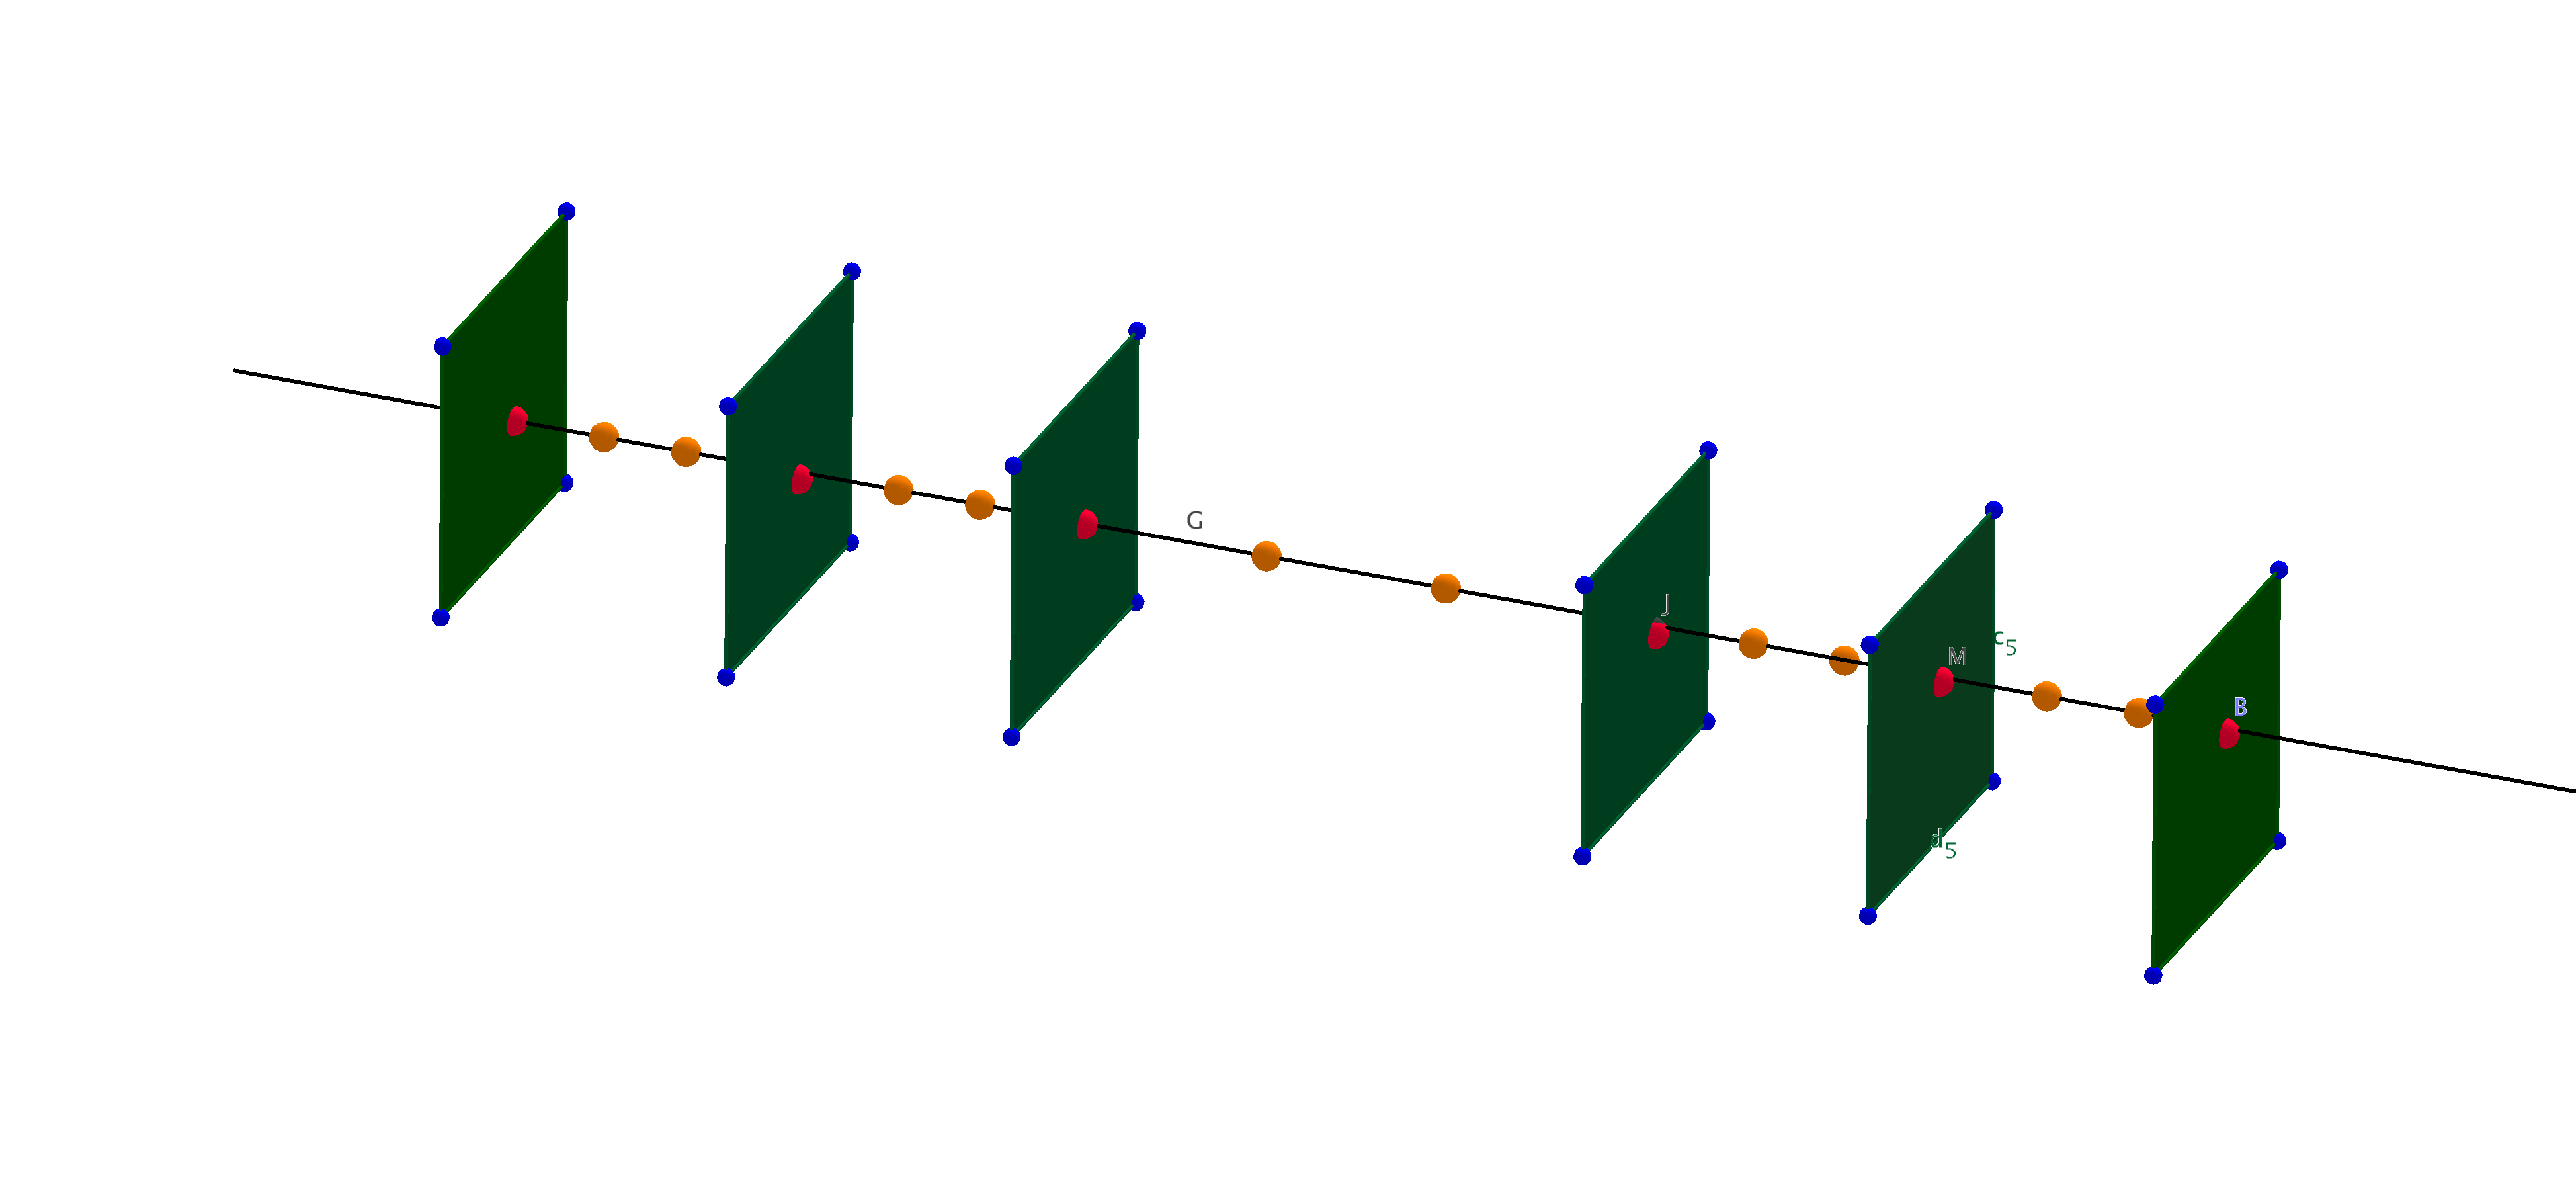
\includegraphics[width=1.0\linewidth]{figures/meas-scat-jac-link.png}
\captionof{figure}{\color{Green} A simple illustration of the linking of discrete points to form a continuous track. The full track does not have to be considered but only the location with measurements and scattering. The red points are measurement/scattering locations, the orange are only scattering.  All the points are linked together by Jacobians which are determined from the initial trajectory. The location of the points is not correct in the diagram and depends on the material distribution for each setup.}
\label{Scat}
\end{center}
\section*{ATLAS Pixels}
One example of the various ATLAS pixels sensors reconstructed is the Quad module. The Quad module is a large area sensor that is compatible with the geometry of the outer barrel layers and forward disks of the upgraded pixel tracker. It is readout with the 4 FEI4s with 50x250 $\mu m^2$ pixel size\cite{quad}. The space inbetween the 4 FEI4s is bridged with ganged pixels. 

\begin{center}
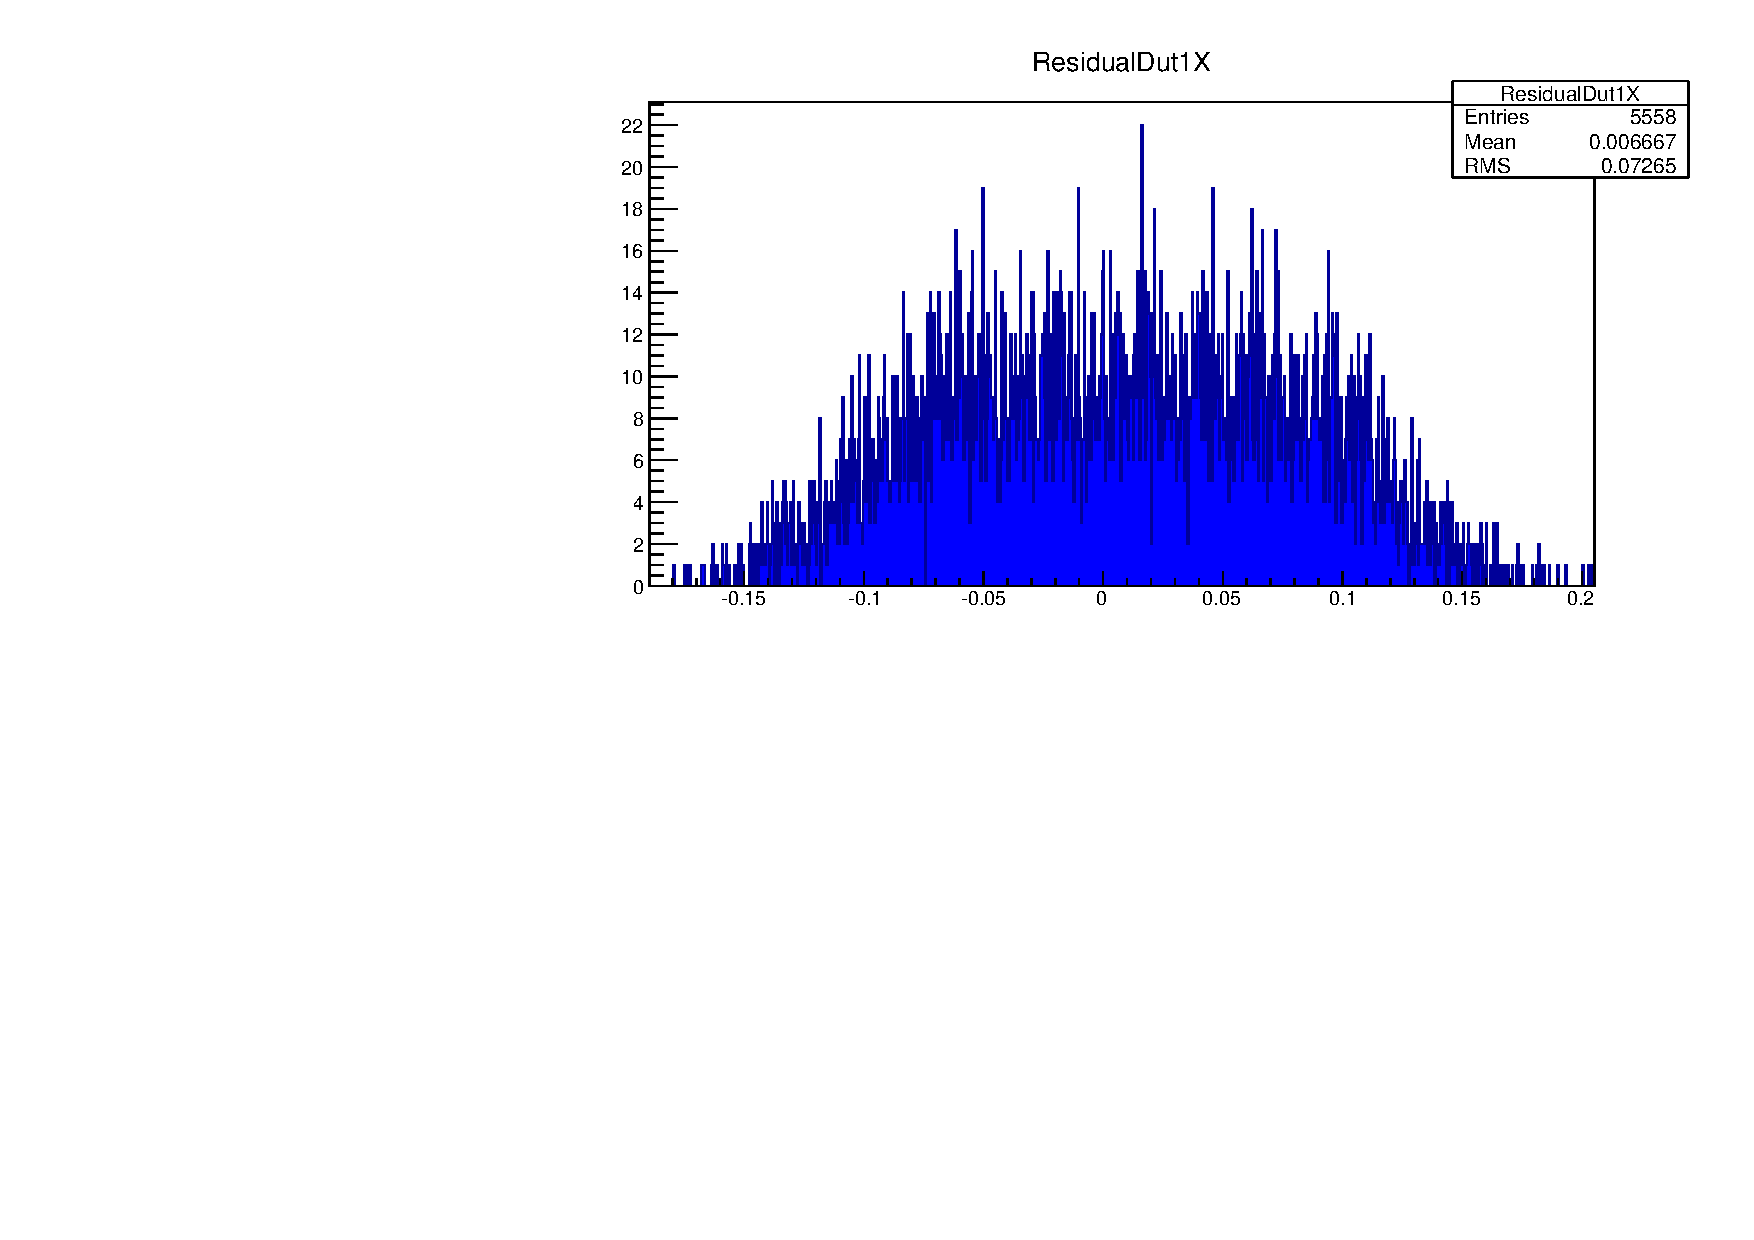
\includegraphics[width=0.8\linewidth]{figures/QuadXRes21.pdf}
\captionof{figure}{\color{Green} Quad module local X axis residual for DESY 4 GeV beam. This fit with the expected 250 $\mu m$ pitch assuming a uniform distribution of predicted hits on each pixel.}
\label{trine}
\end{center}



%\section*{ATLAS Pixels}
 %Two 50x250 $\mu m^2$ FEI4 device was placed in cooling box for measurements at the DESY testbeam. The total radiation length of the box contributed 22% radiation length to the trajectory of the electrons passing through the DUTs. This radiation length must be included in the fit for an accurate model of the track. This is included in the orange points in figure \cite{Scat} between the DUTs and the mimosa planes. 
%\begin{center}
%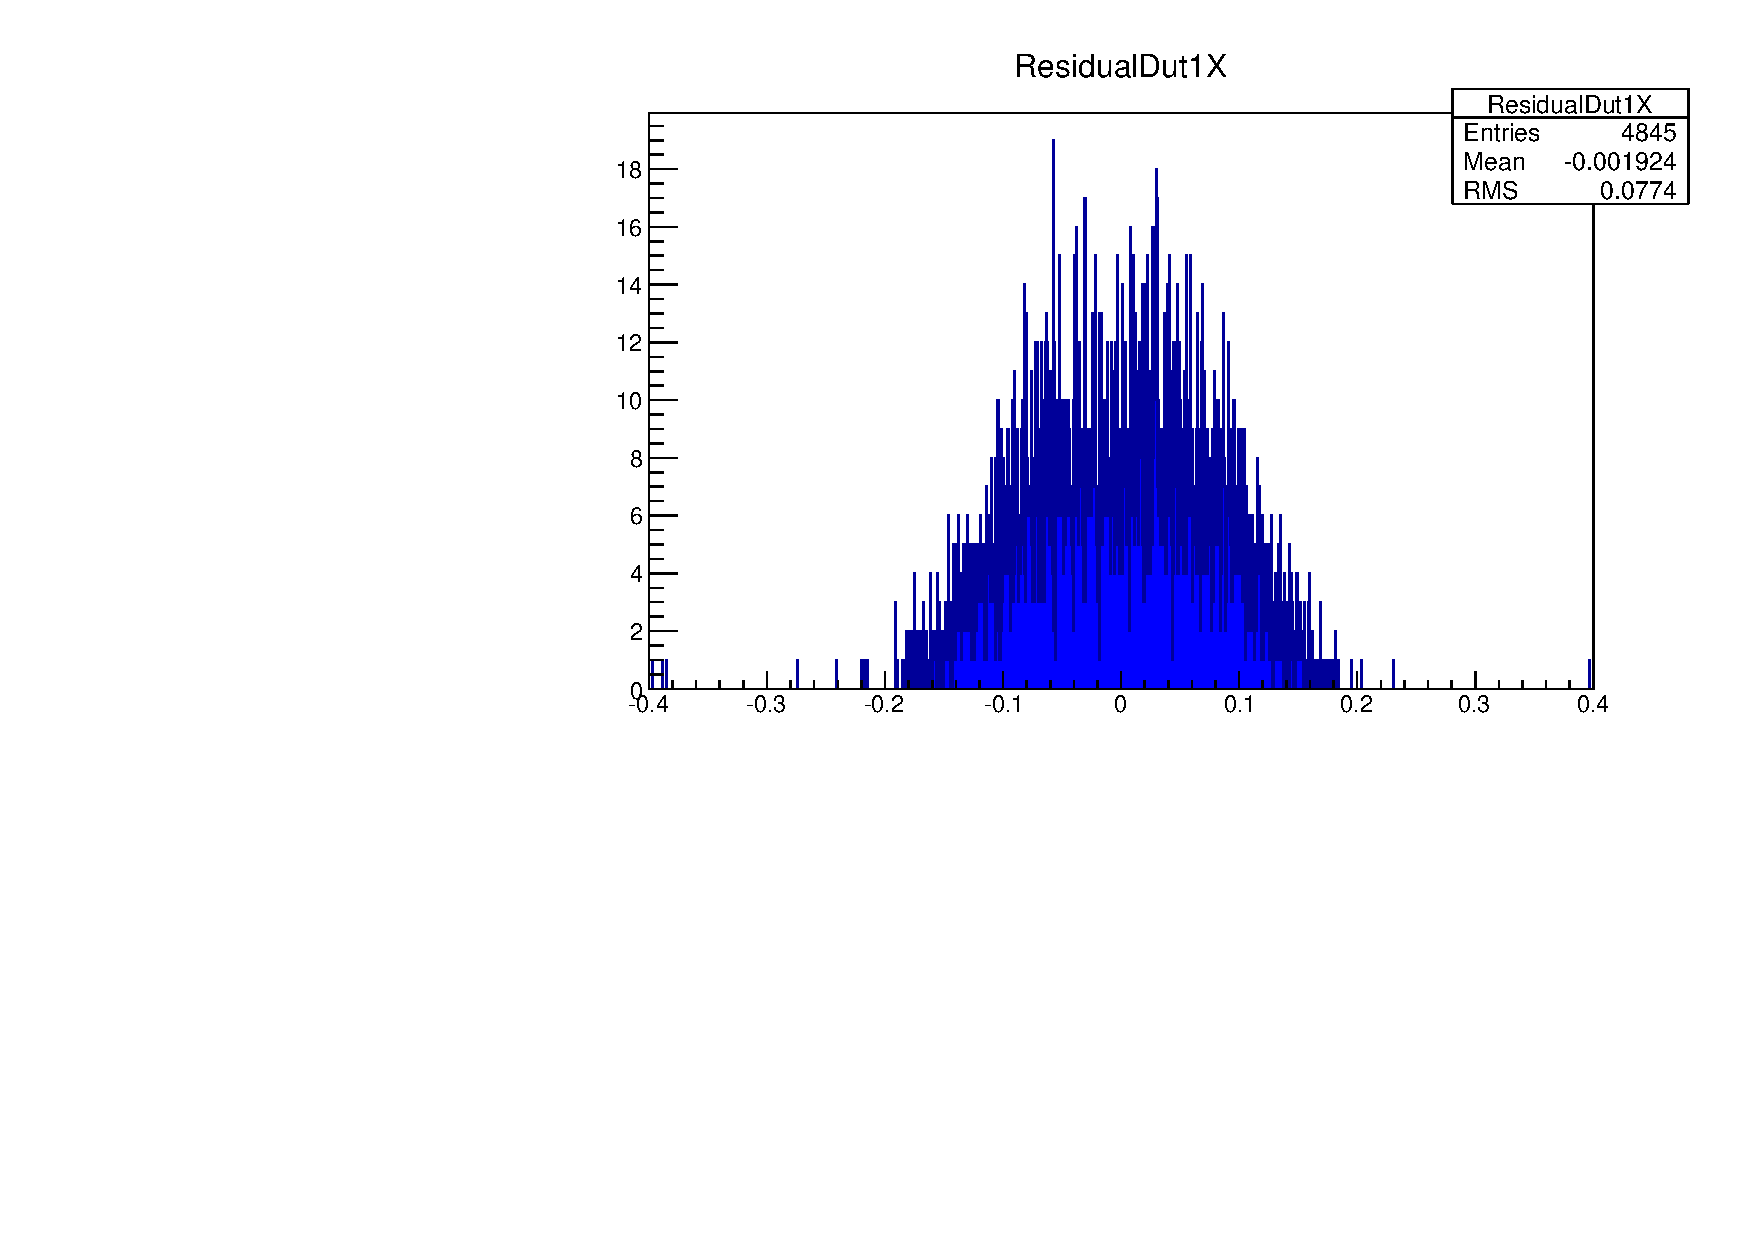
\includegraphics[width=0.7\linewidth]{figures/resXpixel.pdf}
%\captionof{figure}{\color{Green} Quad module local Y axis residual for DESY 4 GeV beam}
%\label{trine}
%\end{center}

\section*{ATLAS strips}
The ATLAS12 sensor is a n$^+$-in-p strip sensors of pitch 70 $\mu m$\cite{atlas12}. 
\begin{center}
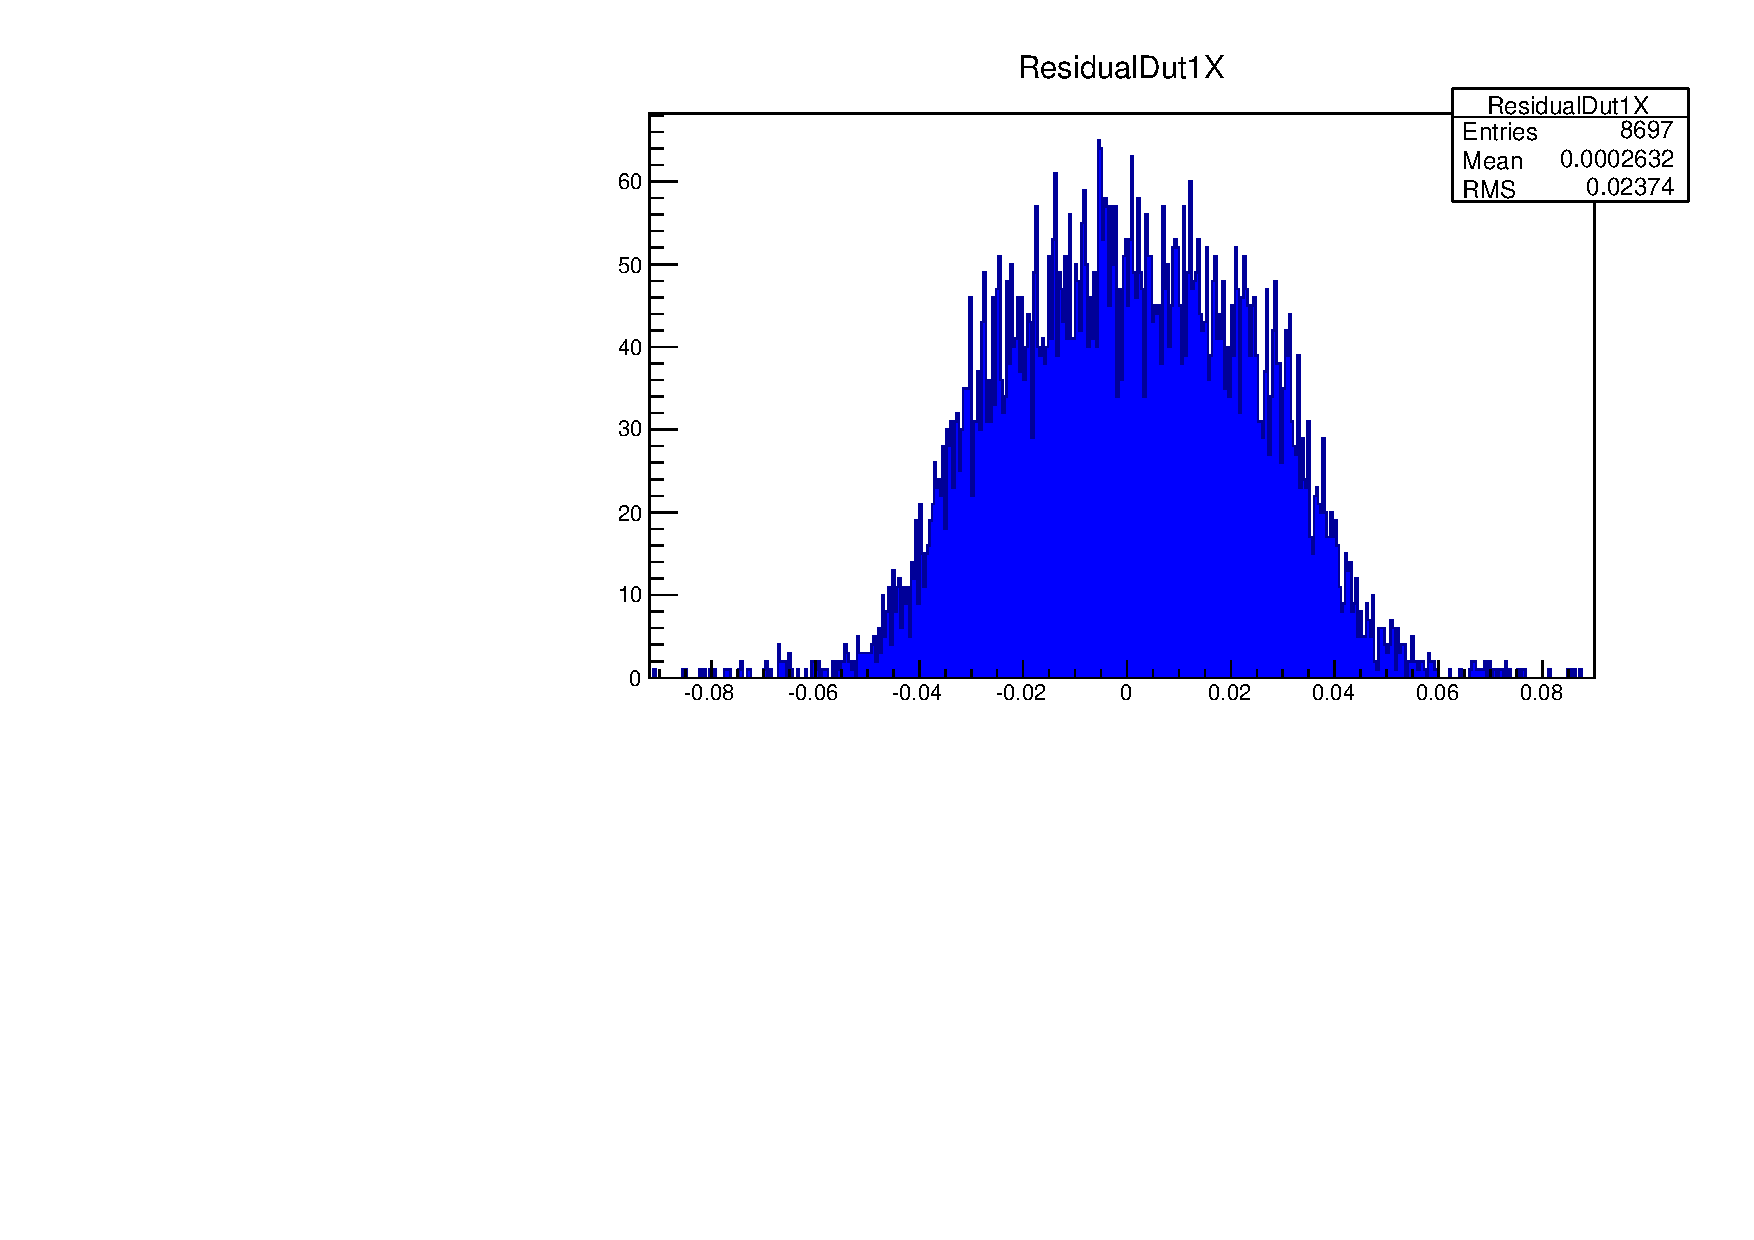
\includegraphics[width=0.7\linewidth]{figures/Res1D.pdf}
\captionof{figure}{\color{Green} This dataset was taken at DESY with beam energy 4.4 GeV. The residual in the X axis local frame. The local frame is the one with the X axis perpendicular to the X axis. This sensor has not undergone full body alignment due to large correlations in the rotations round the X/Y axis and Z shifts. This is due to the large offsets of the hit strips in the local frame. The beam divergence of the DESY beam is approximately 1.5 $\mu$Rad, therefore these rotations are weak modes relative to the tracks fit characterized by the chi2 test statistic . }
\label{strip}
\end{center}


\section*{Additional features}
This track fitting procedure has been used for many different purposes. Some are complete and others are in development. In all cases examples from the raw data to the final reconstructed tracks are available as part of the EUTelescope examples. 

The fitter has been tested with use in a magnetic field with various beam energies at the DESY testbeam. Both forms of pattern recognition are designed to function in the presence of magnetic fields. The energy of each track is assumed constant which is an approximation since this will change during the tracks trajectory.
\begin{center}
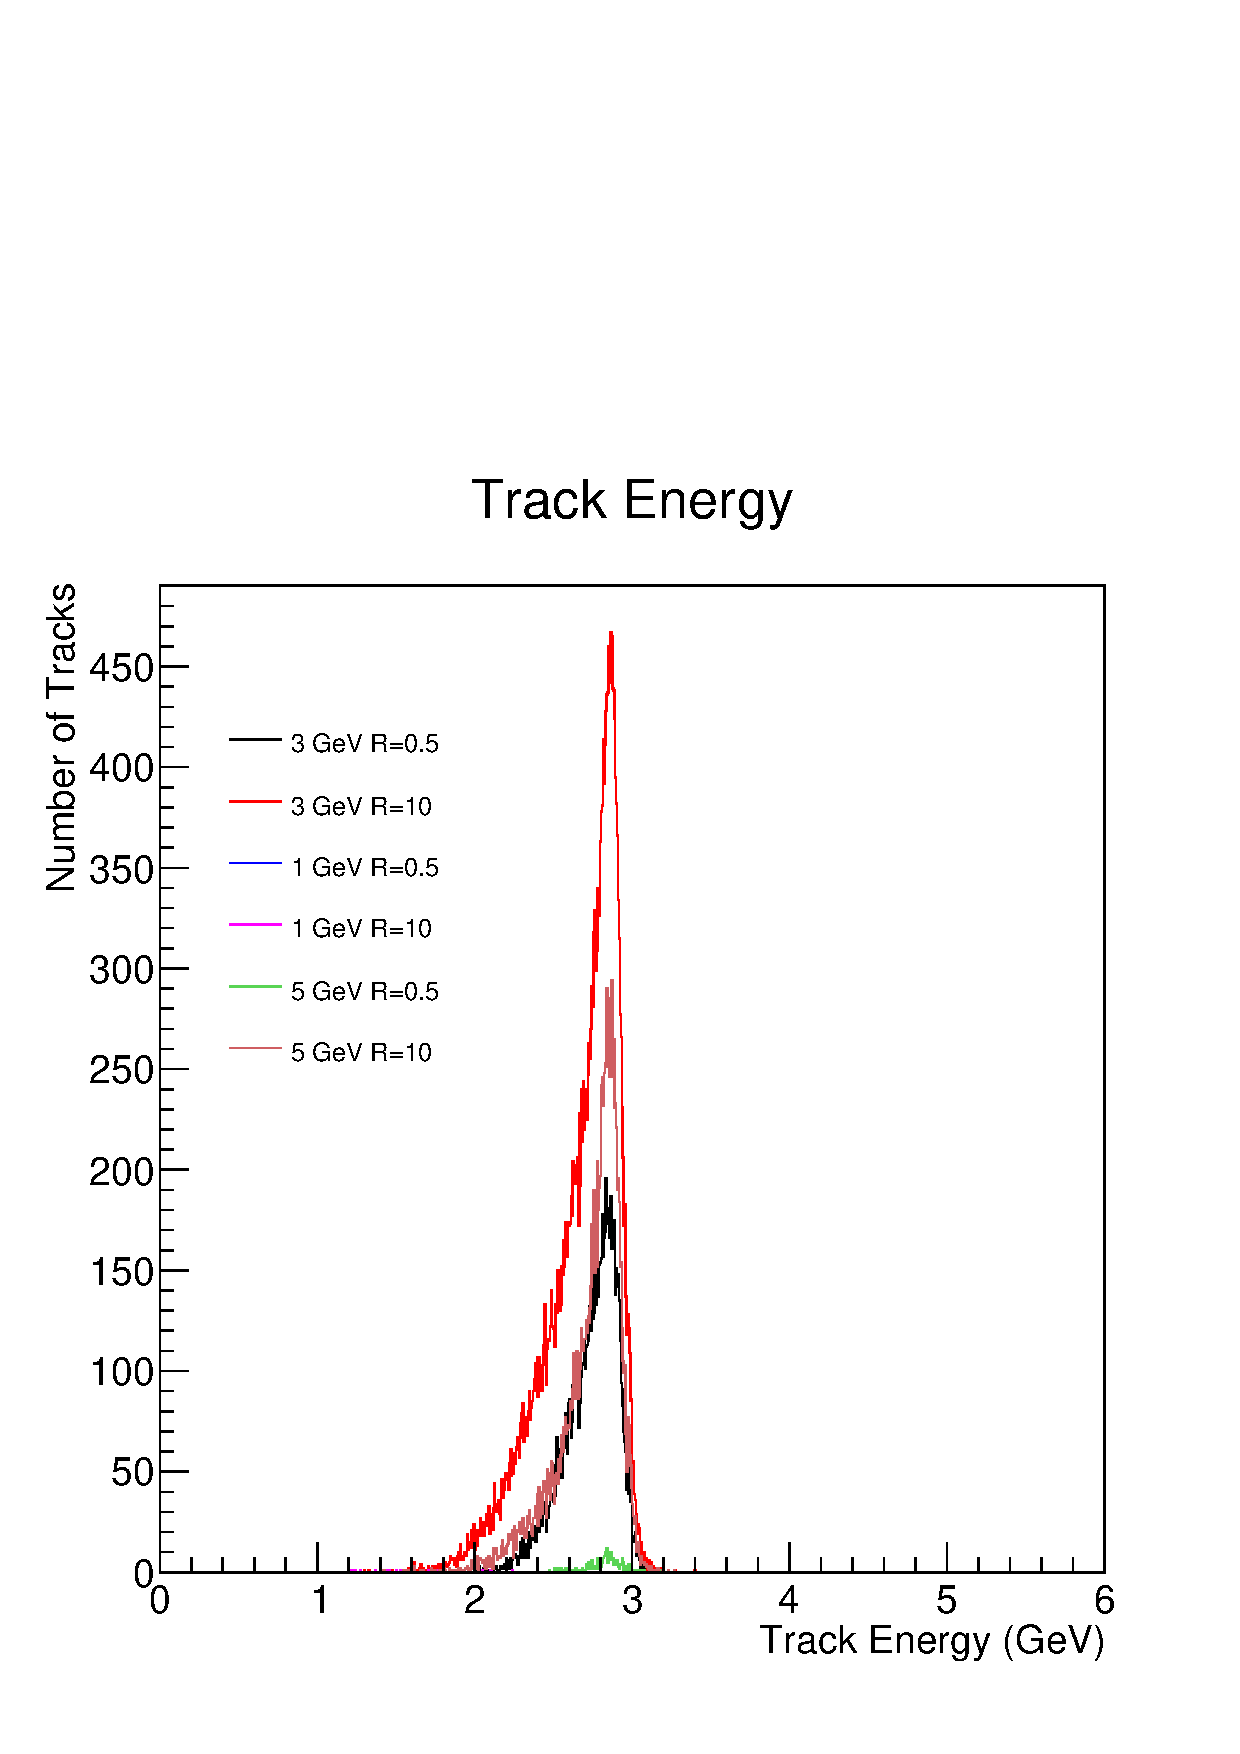
\includegraphics[width=0.8\linewidth]{figures/beamE3B1.pdf}
\captionof{figure}{\color{Green} Measurement of beam energy using the curvature of the beam with 1T magnetic field. The clustering pattern recognition was used to find tracks to be fitted. The R parameter is the clustering window in which hits will be assumed to form a track if within this window. No bias was found between pattern recognition settings and the final measured beam energy.}
\label{trine}
\end{center}

A range of beam energies (1 GeV to 5 GeV)/magnetic fields (0 T to 1 T) from different datasets have been fitted and aligned. The estimated track energies have all corresponded to expected physical values given some energy loss due to bremsstrahlung and the nature energy spread of the beam.

A scattering plane of interest can be placed at any location using the geometry description with EUTelescope. This allows the scattering at a location in space to be estimated using the kink angles at that location. This is currently been used for radiation length measurements and in development. 

A ATLAS12 sensor has been reconstructed using the ALiBaVa readout system. This allows the charge information to be determined, this reduces the value of the measured uncertainty of hit position. 

\begin{thebibliography}{9}
	\bibitem{quad} P.P AllPort et al. "Development of planar pixel modules for the ATLAS high luminosity LHC tracker upgrade".Nuclear Instruments and Methods in Physics Research Section A: Accelerators, Spectrometers, Detectors and Associated Equipment 2014: 109–113 
	\bibitem{atlas12} Unno, Y. et al, "Development of n$^+$-in-p large-area silicon microstrip sensors for very high radiation environments – ATLAS12" design and initial results. Proceedings, 9th International Symposium on Development and Application of Semiconductor Tracking 2014:80-90 
\bibitem{eutel} EUTelescope 1.0: Reconstruction Software for the AIDA Testbeam Telescope. Bisanz T, Morton A, Rubinskiy I, Cern document server

	\bibitem{claus1}  C. Kleinwort, General Broken Lines as advanced track model, Draft Manual, DESY, 2011
                        Detectors (HSTD-9)
	\bibitem{claus2}  C. Kleinwort, General Broken Lines as advanced track fitting method, NIM A, 673 (2012), 107-110
%	\bibitem{blobel} V. Blobel, Millepede II. https://www.wiki.terascale.de/index.php/Millepede_II. (obtained 2 September 2013)
\end{thebibliography}

\section*{Acknowledgements}
Thanks to Craig Buttar, Kenneth Wraight and Andy Blue for helping with much of the reconstruction before pattern recognition, track fitting and alignment. Thanks to Claus Kleinwort who has taught me almost everything about track fitting and alignment. 



%----------------------------------------------------------------------------------------

\end{multicols}
\end{document}
